\chapter{Technical overview}

The developement of the MMU for 3D printer requires an understanding of several key concepts and technologies. This chapter aims to provide the neccessary background and context to better understand the MMU implementation discussed in later chapters. Even for those already familiar with the subject, a brief refresher might be helpful.

\section{Understanding 3D print technology}

Let us start with what 3D print is and what it does.
3D printing technology, also known as additive manufacturing, enables the creation of three-dimensional objects by layering materials based on digital models. This process has unlocked new avenues for innovation, allowing designers, engineers, and hobbyists to bring their ideas to life in a tangible form. In this chapter, we will delve into the fundamentals of 3D printing technology, with a focus on the popular Fused Deposition Modeling (FDM) method utilized in Prusa 3D printers. By understanding the underlying principles of FDM technology.

\section{Fused Deposition Modeling}

Fused Deposition Modeling (FDM) \cite{fdm} technology has revolutionized manufacturing and prototyping by offering a cost-effective and accessible method for creating three-dimensional objects. By understanding the principles of FDM printing, users can harness the full potential of this technology to bring their ideas to life with precision and efficiency.

Advantages of FDM Technology are cost-effectiveness: FDM printers are relatively affordable compared to other 3D printing technologies, making them accessible to a wide range of users, FDM printers are user-friendly and require minimal setup, making them ideal for beginners and experienced users alike, FDM enables rapid iteration and prototyping, allowing designers to quickly test and refine their ideas.

\subsection{Printing process}

\subsubsection{Slicing for FDM}
The process begins with the creation or acquisition of a 3D model in a computer-aided design (CAD) software. The model is then exported as a STL \cite{stl} file, which contains the geometric information needed for printing.
Slicing software, such as PrusaSlicer \cite{slicer}, processes the STL file and generates a G-code \cite{gcode} file containing detailed instructions for the printer's movements, such as the path the print head should follow, the amount of filament to extrude, and the temperature settings

\subsubsection{Printing}
Once the slicing is complete, the sliced file is transferred to the 3D printer. The printer heats the thermoplastic filament to its melting point and extrudes it through the nozzle onto the build platform. The nozzle moves in accordance with the instructions from the sliced file, depositing each layer of material until the object is fully formed. After printing, the object may require post-processing steps such as removing support structures.


\section{Extruder}

Understanding the extruder component is crucial for a MMU project because it directly influences material handling, filament control, compatibility, software integration, and troubleshooting. Extruder, see Figure~\ref{fig:extruder}, is responsible for pushing filament through the hotend, melting it, and depositing it onto the print bed. In an MMU setup, where multiple filaments are used, knowing the extruder helps in handling different materials effectively. It ensures proper control over filament flow, enabling smooth transitions between materials. Different extruders have varying capabilities and limitations, making it essential to select the right one for the MMU project \cite{3d-print-basics}. Understanding the extruder is particularly vital when implementing a new MMU system, as it lays the groundwork for optimizing the mechanical and electronic coordination required for managing multiple materials. This knowledge aids in integrating it with software systems for coordinated filament loading and switching. Moreover, troubleshooting issues like under-extrusion or jamming requires knowledge of the extruder's operation to diagnose and resolve problems efficiently. Overall, a comprehensive understanding of the extruder is essential for a successful implementation and operation of the MMU project, ensuring high-quality prints with multiple materials.

\begin{figure}[ht]
    \centering
    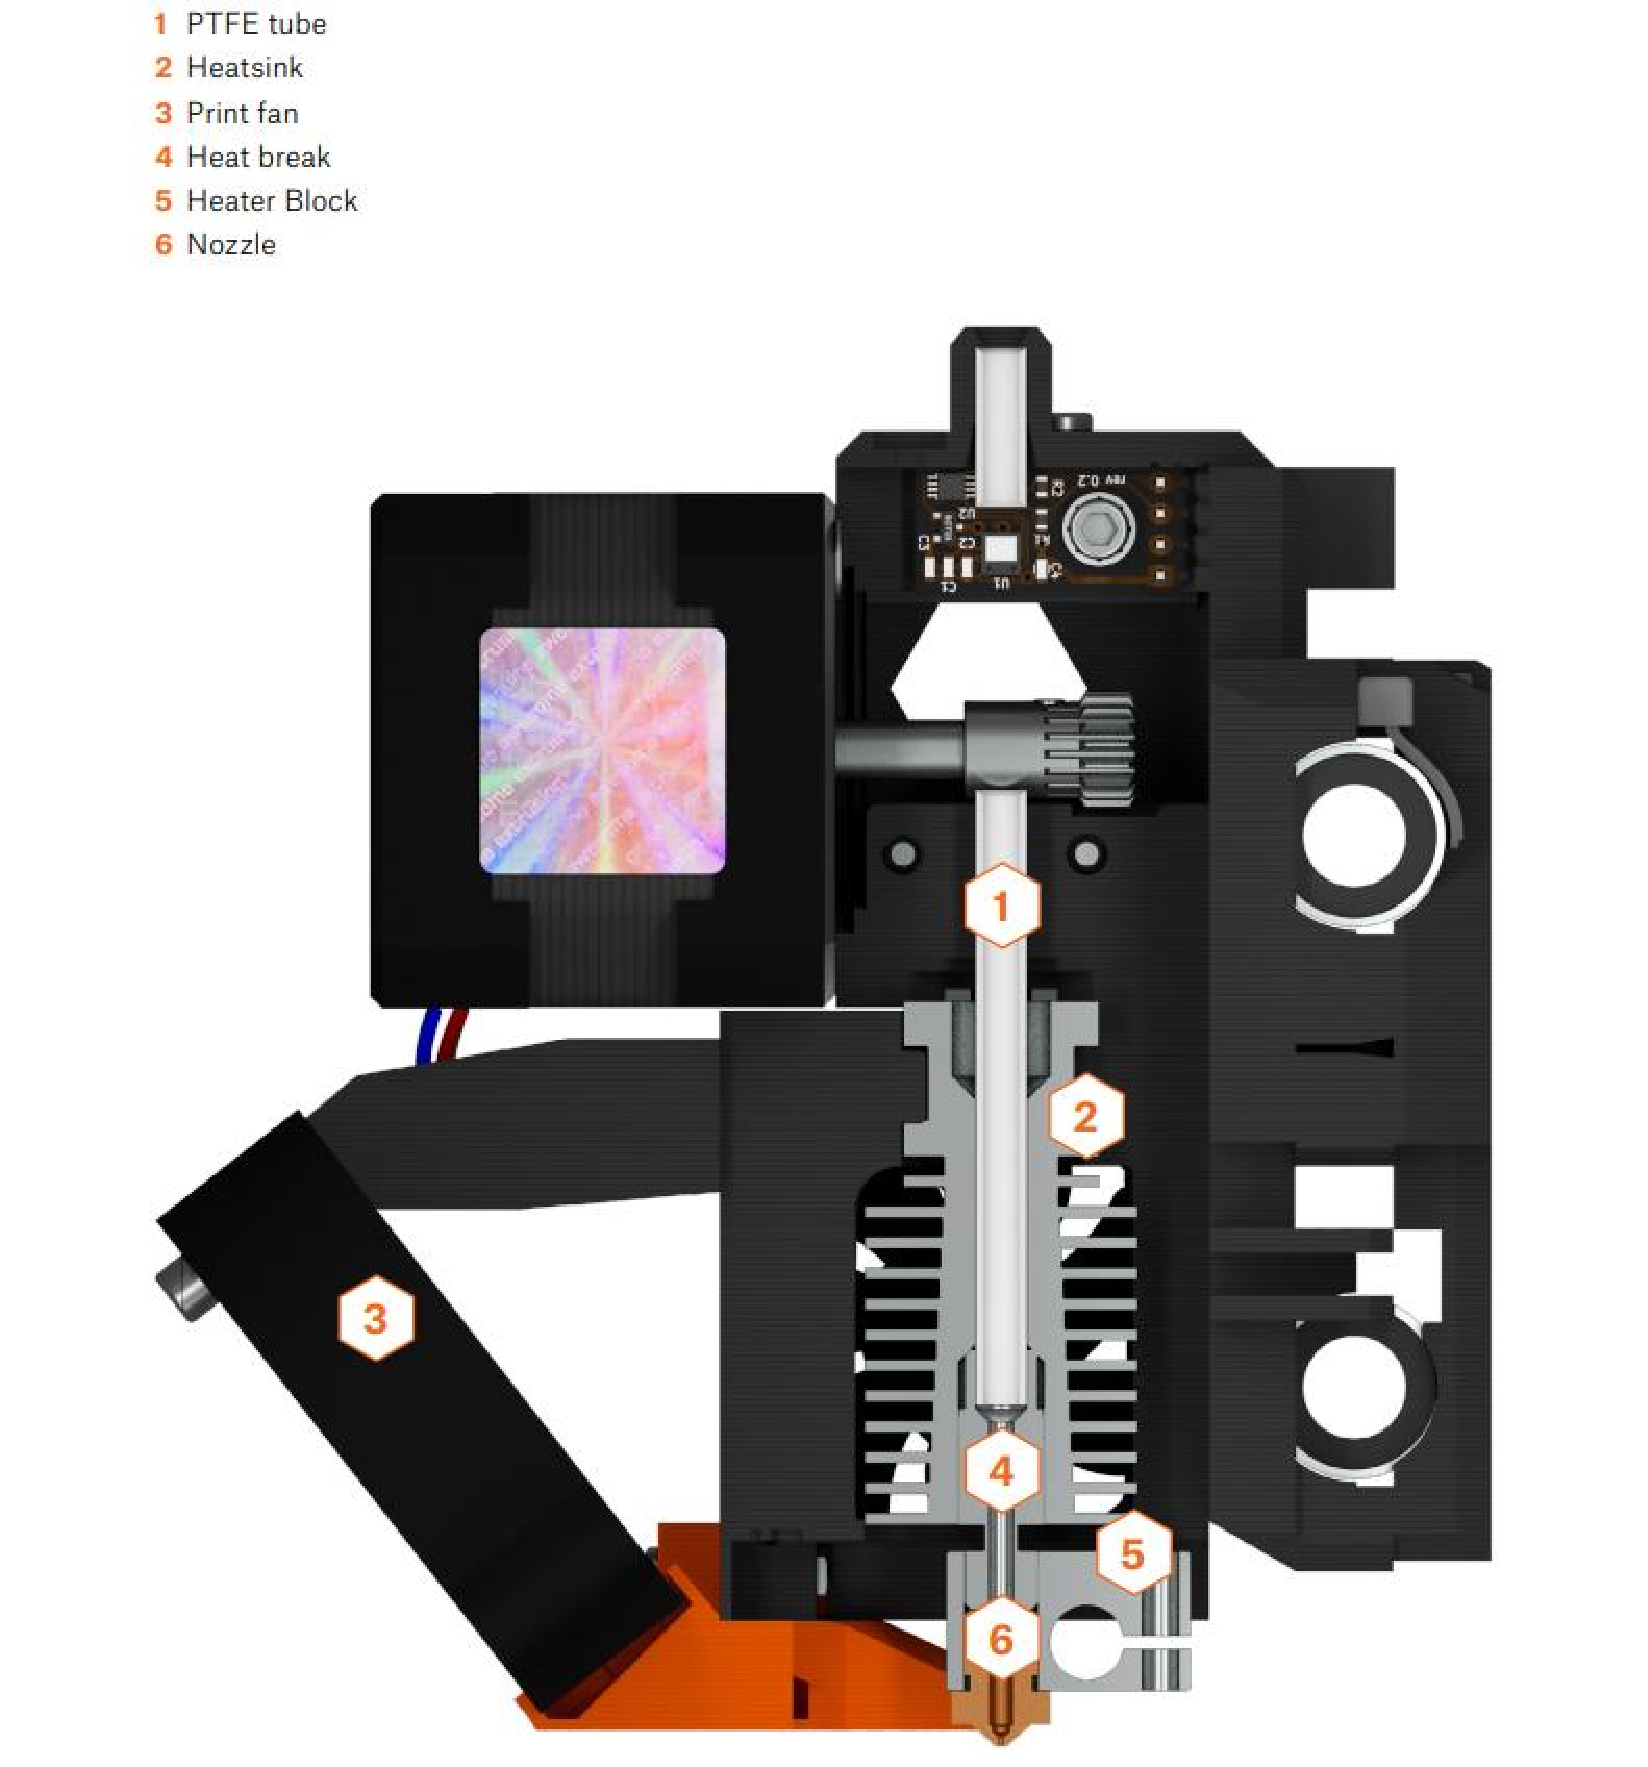
\includegraphics[width=0.8\linewidth]{img/extruder_prusa}
    \caption{Detail of the extruder}
    \label{fig:extruder} 
\end{figure}

\subsection{Heatsink}

The heatsink is part of the extruder that dissipates heat away from the hotend, preventing the filament from melting too early as it travels down the extruder assembly. It is usually attached directly above the heat break and features fins or ridges to increase the surface area, improving its ability to cool by air flow provided by the print fan.

\subsection{Print fan}

The print fan is designed to blow air directly onto the printed material as it exits the nozzle, helping in cooling the material immediately after deposition. This rapid cooling is essential for preventing warping and ensuring good adhesion between layers.

\subsection{Heat break}

The heat break is a narrow and often thermally conductive component that connects the heatsink and the heater block. Its primary function is to restrict the flow of heat upwards, ensuring the filament remains solid until it reaches the heater block, which is critical in maintaining consistent extrusion and preventing jams.

\subsection{Heater block}

The heater block is a metal block that surrounds the heat break and houses the heating element and temperature sensor. Its primary role is to evenly distribute heat to melt the filament precisely before it is pushed through the nozzle. The block maintains a consistent temperature.

\subsection{Nozzle}

The nozzle is the component at the very tip of the extruder that directs the molten filament onto the print bed. Nozzles come in various diameters which influence the resolution and speed of printing; smaller nozzles produce finer details, while larger nozzles allow for faster print speeds

\subsection{Polytetrafluoroethylene tube}

The Polytetrafluoroethylene (PTFE) tube \cite{ptfe} guides the filament from the filament spool to the hotend. It minimizes friction due to its low coefficient of friction, allowing for easier and more reliable filament feeding.

\section{Physics backround}

In this section, we will focus on the fundamental principles of DC motors and Hall effect, which are two pivotal concepts MMU hardware system is based on. 

\subsection{Direct current motor principle}

Direct current (DC) motor is a type of electrical machine that converts electrical energy into mechanical energy through the interaction of magnetic fields. It works on the principle of the Lorentz force, which states that a current-carrying conductor placed within a magnetic field experiences a force. This fundamental principle is harnessed in a DC motor to produce rotational motion.

When a DC motor is powered, an electric current flows through the armature coil. The magnetic field produced by the stator interacts with the magnetic field generated by the electrified armature. According to the left-hand rule of Fleming, which predicts the direction of the force acting on a current-carrying conductor in a magnetic field, this interaction creates a force perpendicular to both the direction of the current and the magnetic field. This force generates torque at the armature, causing it to spin.
A
DC motors are valued for their simple design and easy control, high reliability and torque at low speeds, and cost-effectiveness across a wide range of applications \cite{dc-motor}.

\subsection{Hall effect}

The Hall effect occurs when an electric current flows through a conductor with a magnetic field applied perpendicular to the current. This interaction generates a voltage across the conductor, which is perpendicular to both the current and the magnetic field. The Hall effect is useful for measuring magnetic field strength and determining the type of charge carried in a material. It is also employed in various devices like Hall effect sensors, which are used to measure magnetic fields, speed, and proximity in many applications \cite{hall-effect}.
